\documentclass[tikz,border=6pt]{standalone}
\usepackage[utf8]{inputenc}
\usepackage[T1]{fontenc}
\usepackage{amsmath,amssymb}
\usepackage{lmodern}
\usetikzlibrary{arrows.meta}

\definecolor{ink}{HTML}{1d1d1f}
\definecolor{sub}{HTML}{515154}
\definecolor{muted}{HTML}{6e6e73}
\definecolor{green}{HTML}{1a7f37}
\definecolor{greenbright}{HTML}{30d158}
\definecolor{greenfill}{HTML}{dcf7e3}
\definecolor{red}{HTML}{d70015}
\definecolor{redbright}{HTML}{ff453a}
\definecolor{redfill}{HTML}{ffe5e3}

\begin{document}
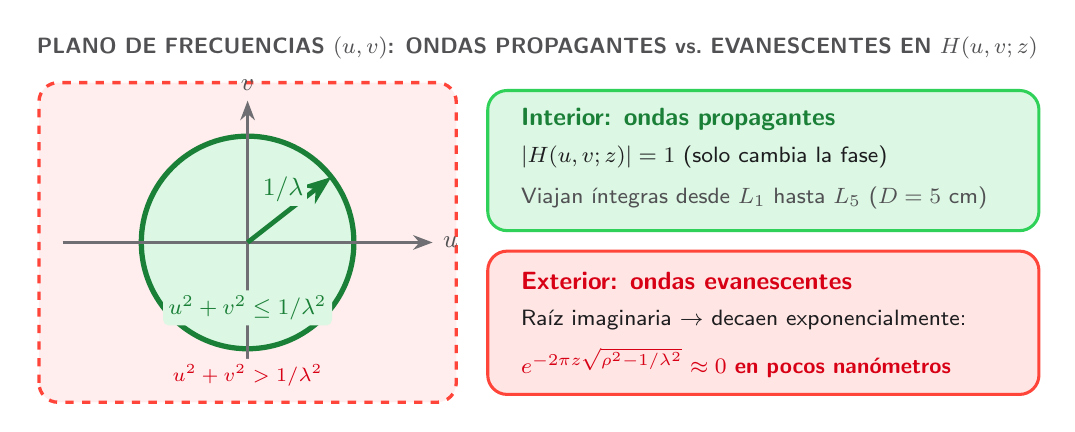
\begin{tikzpicture}[font=\sffamily,>=Stealth]

\node[anchor=west,font=\sffamily\bfseries\footnotesize,text=sub] at (0,4.72)
  {PLANO DE FRECUENCIAS $(u,v)$: ONDAS PROPAGANTES vs.\ EVANESCENTES EN $H(u,v;z)$};

% Zona exterior evanescente
\draw[redbright,dashed,fill=redfill!65,rounded corners=7pt,line width=1.2pt]
  (0.15,0.22) rectangle (5.45,4.28);

% Disco propagante u^2+v^2 <= 1/lambda^2
\filldraw[fill=greenfill,draw=green,line width=1.9pt]
  (2.80,2.25) circle (1.35cm);

% Ejes u, v
\draw[->,muted,line width=0.9pt] (0.45,2.25) -- (5.15,2.25) node[right,font=\sffamily\small\bfseries,text=sub]{$u$};
\draw[->,muted,line width=0.9pt] (2.80,0.45) -- (2.80,4.05) node[above,font=\sffamily\small\bfseries,text=sub]{$v$};

% Radio 1/lambda (evita cruce con texto)
\draw[->,green,line width=1.7pt] (2.80,2.25) -- ({2.80 + 1.35*cos(38)}, {2.25 + 1.35*sin(38)});
\node[fill=greenfill,inner sep=1.5pt,font=\sffamily\small\bfseries,text=green] at (3.25,2.92) {$1/\lambda$};
\node[fill=greenfill,inner sep=2pt,rounded corners=2pt,font=\sffamily\footnotesize\bfseries,text=green] at (2.80,1.42)
  {$u^2 + v^2 \le 1/\lambda^2$};

% Etiqueta exterior
\node[fill=redfill!65,inner sep=2pt,rounded corners=2pt,font=\sffamily\scriptsize\bfseries,text=red] at (2.80,0.56)
  {$u^2 + v^2 > 1/\lambda^2$};

% Cajas explicativas derecha (más anchas para margen holgado)
\draw[greenbright,fill=greenfill,rounded corners=7pt,line width=1.1pt]
  (5.85,2.40) rectangle (12.85,4.18);
\node[anchor=west,font=\sffamily\small\bfseries,text=green] at (6.15,3.82)
  {Interior: ondas propagantes};
\node[anchor=west,font=\sffamily\footnotesize,text=ink] at (6.15,3.34)
  {$|H(u,v;z)| = 1$ (solo cambia la fase)};
\node[anchor=west,font=\sffamily\footnotesize,text=sub] at (6.15,2.82)
  {Viajan íntegras desde $L_1$ hasta $L_5$ ($D = 5\text{ cm}$)};

\draw[redbright,fill=redfill,rounded corners=7pt,line width=1.1pt]
  (5.85,0.32) rectangle (12.85,2.14);
\node[anchor=west,font=\sffamily\small\bfseries,text=red] at (6.15,1.76)
  {Exterior: ondas evanescentes};
\node[anchor=west,font=\sffamily\footnotesize,text=ink] at (6.15,1.26)
  {Raíz imaginaria $\rightarrow$ decaen exponencialmente:};
\node[anchor=west,font=\sffamily\footnotesize\bfseries,text=red] at (6.15,0.72)
  {$e^{-2\pi z\sqrt{\rho^2 - 1/\lambda^2}} \approx 0$ en pocos nanómetros};

\end{tikzpicture}
\end{document}
